%%%%%%%%%%%%%%%%%%%%%%%
%%%%%%%% EPL %%%%%%%%%%
%%%%%%%%%%%%%%%%%%%%%%%

\documentclass[doublecol,final]{epl2}

\usepackage{amsmath}
\usepackage{amssymb}

\makeatletter
\setlength\arraycolsep{2pt}
\makeatother

\vol{110}
\issue{1}
\year{2015}
\firstpage{1}
\doi{10.1209/0295-5075/110/24001}
\pgid{24001}
\received{24 December 2014}
\acceptedinfinalform{7 April 2015}
\paperpub{April 2015}
\onlinepub{29 April 2015}

\title{Leidenfrost drops: Effect of gravity\vspace*{-2pt}}

\shorttitle{Leidenfrost drops: Effect of gravity}

\author{L. Maquet\inst{1}, M. Brandenbourger\inst{1}, B. Sobac \inst{2}, A.-L. Biance\inst{3}, P. Colinet\inst{2} \and S. Dorbolo\inst{1}}

\shortauthor{L. Maquet \etal}

\institute{
\inst{1} GRASP, D\'epartement de Physique B5, Universit\'e de Li\`ege - B-4000 Li\`ege, Belgium\\
\inst{2} TIPs, Fluid Physics Unit, Universit\'e Libre de Bruxelles - C.P. 165/67, B-1050 Bruxelles, Belgium\\
\inst{3} Institut Lumi\`ere Mati\`ere, UMR5306 CNRS, Universit\'e Claude Bernard Lyon 1\\ F-69622 Villeurbanne CEDEX, France
}

\pacs{47.55.D-}{Drops and bubbles}
\pacs{47.55.dp}{Cavitation and boiling}
\pacs{47.15.gm}{Thin film flows}

\abstract{~A specific experimental set-up has been installed in a large centrifuge facility in order to study different aspects of Leidenfrost drops under high-gravity conditions (5,~10, 15 and 20 times the Earth gravity). In particular, the drop lifetime and more precisely the variations of drop diameter \textit{vs.} time have shown to be in good agreement with previous experiments and scaling analysis (\textsc{Biance A.-L.} \textit{et~al.}, \textit{Phys. Fluids}, \textbf{15} (2003) 1632). Moreover, so-called \textit{chimneys} are expectedly observed in the large puddles, the distance between two chimneys depending linearly on the capillary length. Finally, the Leidenfrost point, \textit{i.e.} the temperature above which the Leidenfrost effect takes place, was unexpectedly found to increase slightly with gravity. A~qualitative explanation based on a refined model (\textsc{Sobac B.} \textit{et~al.}, \textit{Phys. Rev. E}, \textbf{90} (2014) 053011) recognizing the non-trivial shape of the vapor film under the drop is proposed to explain this observation.}

\begin{document}

\maketitle

\section{Introduction}

Cooling down a hot body is generally possible by immersing it into a high-heat-capacity liquid such as water. However, if its temperature is too high, the cooling efficiency is dramatically reduced by the instantaneous generation of an insulating vapor layer between the liquid and the hot body~\cite{epl17032bib1}. On a small scale, this phenomenon can rather be taken as an advantage. When a drop is released on a plate heated well above the boiling temperature of the liquid, the drop may levitate on its own vapor. This phenomenon, named Leidenfrost effect after the name of its discoverer~\cite{epl17032bib2}, prevents the drop from touching the substrate, mimicking a non-wetting situation when static effects are considered and a frictionless one when dynamics is investigated. A classical work highlighting the main scaling laws applying to Leidenfrost droplets has been published by Biance \textit{et~al.}~\cite{epl17032bib3}.

In static situations, the shape of the drop and the evaporation dynamics have been recently revisited~\cite{epl17032bib4,epl17032bib5,epl17032bib6,epl17032bib7,epl17032bib8}, highlighting a pocket-like geometry of the vapor film underneath the evaporating drop. Accurate interferometric measurements of the vapor film thickness profile~\cite{epl17032bib9} indeed turn out to be in very good agreement with a \nobreak{theoretical} modeling coupling vapor flow, capillarity and hydrostatic pressure effects~\cite{epl17032bib8}. For large drops, a \nobreak{critical} radius above which the vapor pocket bursts at the upper part of these drops can be determined~\cite{epl17032bib3,epl17032bib4,epl17032bib8}, very similarly to what happens in the related situation of a drop levitating over blown air~\cite{epl17032bib4,epl17032bib10,epl17032bib11}. In dynamic situations, properties of Leidenfrost drops have also been tested by impacting drops on a hot plate~\cite{epl17032bib12,epl17032bib13,epl17032bib14,epl17032bib15}. Finally, the nearly frictionless motion of Leidenfrost droplets can also lead to the self-propulsion of drops on patterned substrates~\cite{epl17032bib16,epl17032bib17} which enables rapid transport of small objects~\cite{epl17032bib18}. Despite this large amount of work devoted to describe and use Leidenfrost drops, the threshold temperature above which the Leidenfrost effect takes place remains poorly understood~\cite{epl17032bib19}. In particular, experimental data on the different factors influencing this effect are still lacking, even though surface roughness and wetting properties are recognized to affect this threshold temperature significantly~\cite{epl17032bib20,epl17032bib21,epl17032bib22,epl17032bib23,epl17032bib24,epl17032bib25}.


In this work, we have investigated the effect of gravity on different properties of Leidenfrost drops, such as drop geometry and lifetime or chimney appearance. The results obtained are in good agreement with classical scalings of Biance \textit{et~al.}~\cite{epl17032bib3}, based on the assumption of a flat bottom surface of the drop. However, we also observe an \nobreak{unexpected} effect of gravity on the Leidenfrost point, which is tentatively interpreted as a subtle consequence of the non-trivial shape of the vapor film underneath the droplet.

Experiments were performed at the Large Diameter Centrifuge (LDC) facility of ESA, in order to reach 20~times the Earth gravity. The main effect of gravity is to modify the apparent weight of the drop, \textit{i.e.} to affect the capillary length~$a$. Indeed, the capillary length is obtained by comparing capillary and gravity forces: $a=\sqrt{\gamma/\rho g \Gamma}$, where $\gamma$ and $\rho$ are the surface tension and the density of the liquid, $g$ the Earth gravity acceleration and $\Gamma$ the reduced gravity, \textit{i.e.} the ratio between the apparent gravity and the Earth gravity. In zero-$g$ environment, the capillary effects are enhanced and the capillary length $a$ \nobreak{diverges}. On the other hand, high-gravity conditions augment the gravity effect and the capillary length decreases. This situation is particularly interesting regarding the \nobreak{Leidenfrost} effect because, during the evaporation, the drop successively experiences three regimes: very large drop $(R > R_c)$, large drop $(a < R < R_c)$, and small drop $(R < a)$~\cite{epl17032bib3}, where $R_c$ is the critical radius for chimney formation. Importantly, increasing the gravity level is not fully equivalent to working with larger droplets under normal gravity. Even though the Bond number $(R/a)^2$ can reach the same value in both cases, gravity is also expected to modify in a non-trivial way the relative role of evaporation in the vapor film underneath the drop, hence its thickness~\cite{epl17032bib3,epl17032bib8}. How these local modifications affect evaporation rate and film boiling state stability (\textit{i.e.} Leidenfrost point) remains an issue that deserves to be tackled. Thus, the aim of the campaign was to investigate the influence of gravity on: i)~the lifetime of the Leidenfrost drop, ii)~the formation and the size of chimneys in the very large-drop regime and iii) the Leidenfrost point (the temperature beyond which the drop levitates). These measurements allow to test existing scaling laws and more detailed theories indirectly by changing only the gravity, other physical properties remaining identical.

\section{Experimental details}

Figure~\ref{epl17032fig1}(a) represents schematically the Large Diameter Centrifuge (LDC). The LDC is a centrifuge with four-meter--long spinning horizontal arms. At the end of each arm, gondolas are attached. The experiment is placed in one of the \nobreak{gondolas}, inclined due to spinning, and which experiences the \nobreak{apparent} gravity, ${\vec{g}}^{*}$ equal to
\begin{equation}%eq1
\vec{g}^{\ *} = \vec{g} + \omega^{2} R_{g} {\vec{e}}_r, \label{epl17032eqn1}
\end{equation}
where $\omega$ is the angular velocity of the centrifuge, $R_{g}$ the distance between the axis of rotation and the point of interest in the gondola, $\vec{g}$ the Earth gravity and $\vec{e}_r$ the unit vector radial to the movement of the gondola. Hence the reduced gravity is given by $\Gamma = g^*/g$.

A hot plate whose temperature is controlled was \nobreak{embarked} in one of the gondolas of the LDC. The plate was composed of two heat pipes horizontally placed inside an aluminum plate $(130\un{mm} \times 130\un{mm} \times 20\un{mm})$. A~\nobreak{thermocouple} was screwed on the bottom side of the plate. A heating regulator was used to stabilize the temperature of the plate between $50\un{^{\circ}C}$ and $400\un{^{\circ}C}$ with a precision of about $1\un{^{\circ}C}$. A thick aluminum annulus ($75\un{mm}$ of internal diameter, 20\un{mm} of thickness and 30\un{mm} of height) was fixed on the plate (to~prevent the drops from escaping). Drops of controlled volume were produced remotely inside the annulus via a syringe pump. Finally, a camera (Thorlabs, DCU223M) was used to record the drop from the top of the plate at~3 frames per second. All the devices were remotely controlled from the control room of the LDC.

\begin{figure}%f1
\centering
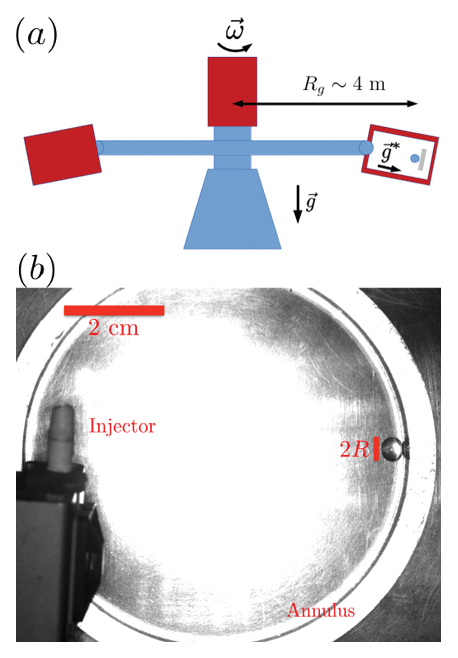
\includegraphics{epl17032f1_pr.eps}
\caption{(Colour on-line) (a) Schematic illustration of the experimental setup. (b) Typical image (top~view). The injector is on the left side. The Leidenfrost drop is on the right side of the annulus. The scale bar represents 2\un{cm}.} \label{epl17032fig1}
\vspace*{-5pt}
\end{figure}

The experimental procedure was the following. The temperature of the plate $T$ and the reduced gravity $\Gamma$ were set to the desired values. After stabilization of both parameters, a water drop with a volume of $0.153 \pm 0.005\un{ml}$ was released on the plate from a height of $\sim 5\un{cm}$. The pictures were taken from the top in order to measure the lifetime $\tau$ and the radius $R$ of the drop. This operation was performed 3~times for each set of control parameters ($T$~and~$\Gamma$). A typical image obtained is shown in fig.~\ref{epl17032fig1}(b). Note that due to the frictionless movement of these drops, they are very sensitive to any angle of the substrate and thus unavoidably tend to stabilize at the lowest point.

A second kind of experiments consists in pouring a large quantity of liquid in the annulus in order to completely fill it. In doing so, we meet conditions to obtain chimneys. Their interdistance $D_{ch}$ can be measured by image \nobreak{analysis}.

\section{Results and discussion}

\subsection{Lifetime vs. gravity}

In fig.~\ref{epl17032fig2}, the measured lifetime of the 0.153\un{ml} water drop has been reported as a function of the difference of temperature between the plate and the drop interface assumed at saturation~\cite{epl17032bib3}, \textit{i.e.} $\Delta T=T-T_{\textit{sat}}$, where $T_{\textit{sat}}$ is the saturation (boiling) temperature ($100\un{^{\circ}C}$ for water). This procedure has been performed for 5~gravity levels.

Let us start by describing the $\Gamma=1$ data. As the temperature of the plate is around $200\un{^{\circ}C}$ , \textit{i.e.} $\Delta T = 100\un{^{\circ}C}$, very short lifetimes are found (of the order of one second ---not recorded). The lifetime dramatically increases above $\Delta T = 115\un{^\circ C}$ as the drop starts levitating. A maximum is reached at $\Delta T = 125\un{^\circ C}$. The Leidenfrost point is defined as the maximum of the drop lifetime as a function of the plate temperature~\cite{epl17032bib1}. Beyond this maximum, the lifetime decreases for higher temperatures. Note that for $\Gamma=1$, the uncertainties on the evaporation time are the largest. When the drop is released, it tends to break up in smaller drops which coalesce back in a time that is decreased when the gravity is increased. For $\Gamma = 1$, this time was typically of a few seconds with a standard deviation of the same order of magnitude. The probabilistic behavior of the coalescence makes it impossible to draw any conclusion on this particular phenomenon with our experiments.

\begin{figure}%f2
\centering
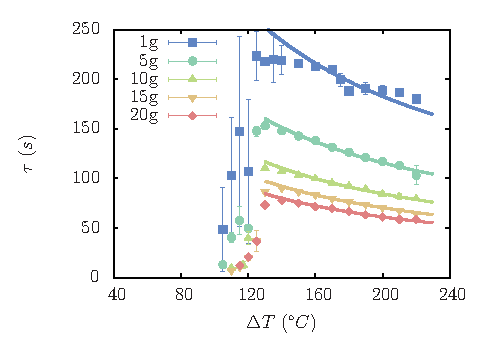
\includegraphics{epl17032f2_pr.eps}
\caption{(Colour on-line) Lifetime of a Leidenfrost drop (of an initial volume $V=0.153\un{ml}$) as a function of the superheat $\Delta T$ for five different apparent gravities $\Gamma g$ (see legend). Points are experimental data. Solid lines are power law fits with \nobreak{exponent}~$-3/4$.} \label{epl17032fig2}
\end{figure}

When gravity is increased, the lifetimes are observed to be shorter. However, a decrease with temperature is still observed, the larger the gravity the slighter the\break decrease.

\begin{figure}%f3
\centering
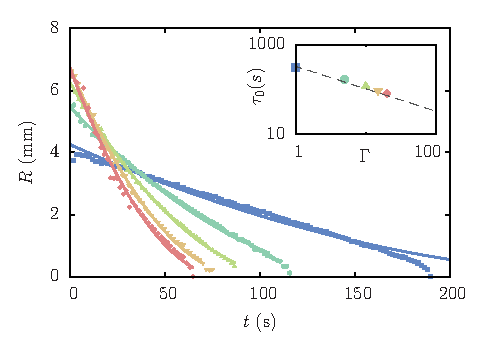
\includegraphics{epl17032f3_pr.eps}
\caption{(Colour on-line) Evolution of the drop radius $R$ as a function of time for five different reduced gravities: $\Gamma=1$, 5, 10, 15 and~20. The temperature of the substrate is $300\un{^\circ C}$. The legend is identical to the one provided in fig.~\ref{epl17032fig2}. The solid lines are fits using eq.~(\ref{epl17032eqn2}) with the evaporation time $\tau_{0}$ as fit parameter. The inset presents $\tau_{0}$ as a function of the reduced gravity $\Gamma$. The dashed line is a power law fit with exponent $-1/2$, \textit{i.e.} $\tau_0 \propto \Gamma^{-1/2}$.} \label{epl17032fig3}
%\vspace*{-5.5pt}
\end{figure}

The radius of the drop $R$ was recorded over time for $\Gamma=1$, 5, 10, 15 and~20 and $\Delta T=200\un{^\circ C}$ in order to \nobreak{capture} the dynamics of evaporation. The data are shown in fig.~\ref{epl17032fig3}. Note that only 20{\%} of the data are presented in order to enable a better visualization of the results. First of all, it turns out that the initial radius $R(0)$ increases with gravity, as expected. Indeed, in a perfect non-wetting situation, the shape of a drop above the capillary length $a$ defined above is the one of a flattened puddle, whose thickness $h$ is set by a balance of gravity and surface tension and is nearly equal to~$2a$~\cite{epl17032bib26}. By assuming that the droplet has a shape of a flat pancake, the volume conservation sets the radius of the droplet to $R(0)=\sqrt{V/2 a \pi} \propto \Gamma^{1/4}$. To be more accurate, the shape of a droplet ``levitating'' on a thin layer of its own vapor has been modeled in more detail~\cite{epl17032bib8}, revealing a more complex shape. The effect of gravity on this shape is presented in fig.~\ref{epl17032fig4} (at~constant volume), showing that the drop is more and more flattened by the increase of the gravity level, changing from a quasi-spherical to a puddle-like shape. As far as the evaporation dynamics is concerned, the radius decreases with time (see fig.~\ref{epl17032fig3}), with a largest rate when the gravity is larger. This effect is attributed to the droplet shape, as when it is squeezed, a larger surface is available for heat transfer, closer to the hot plate in the neck region, thus leading to faster evaporation.

\begin{figure}%f4
\centering
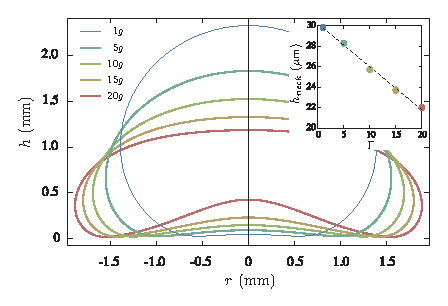
\includegraphics{epl17032f4_pr.eps}
\caption{(Colour on-line) Theoretical shapes of a $10\un{\mu L}$ Leidenfrost drop for five different reduced gravities: $\Gamma=1$, 5, 10, 15 and~20. The temperature of the substrate is $300\un{^\circ C}$. These shapes are numerically determined using the theoretical modeling presented in ref.~\cite{epl17032bib8}. The inset represents the thickness of the vapor film at the location where it is thinnest, $h_{\textit{neck}}$, as a function of the reduced gravity $\Gamma$, using the same model. The dashed line is a guide to the eye.}
\label{epl17032fig4}
\end{figure}

In the case of a drop larger than the capillary length, variations of the radius with time can be captured by a simple modeling~\cite{epl17032bib3}, assuming that the drop is cylindrical and that the vapor layer underneath has an homogenous thickness.~The conductive heat flux through the vapor film generates an evaporation rate balanced by the vapor flux in the lubrication film.~This determines both film thickness and evaporation rate of the droplet, and leads to
\begin{equation}%eq2
R(t)=R(0)\left(1-\frac{t}{\tau_0}\right)^2, \label{epl17032eqn2}
\end{equation}
where $R(0)$ is the initial radius and $\tau_0$ is the evaporation time defined as
\begin{equation}%eq3
\tau_0=2\left(\frac{4\rho aL}{\kappa_v\Delta T}\right)^{3/4}\left(\frac{3\eta_v}{\rho_v \Gamma}\right)^{1/4}{R(0)}^{1/2}={A\ \Delta T^{-3/4}}, \label{epl17032eqn3}
\end{equation}
where $L$ is the latent heat of vaporization of water, $\eta_v$, $\kappa_v$, and $\rho_v$ are the dynamic viscosity, the thermal conductivity and the density of the vapor, respectively (hereafter, all vapor properties are evaluated at its mean temperature $(T+T_{\textit{sat}})/2$). The parameter $A$ gathers the dependence on the initial size of the drop, on the reduced gravity, and on physical properties of the liquid and of the vapor. Note that even though the scaling $\Delta T^{-3/4}$ is indeed coherent with the data of fig.~\ref{epl17032fig2}, the same can be said about the slightly different scaling $\Delta T^{-5/6}$ found by~\cite{epl17032bib8}, given the limited range of values of $\Delta T$ available here.

Fits using eq.~(\ref{epl17032eqn2}) are presented as solid curves in fig.~\ref{epl17032fig3} and also show a good agreement with experimental data. The parameter $\tau_{0}$ is derived from this fit and reported in the inset of fig.~\ref{epl17032fig3}. It turns out that $\tau_{0}$ scales as $\Gamma^{-1/2}$, as also predicted by eq.~(\ref{epl17032eqn3}) in which $R(0) \propto \Gamma^{1/4}$.

Let us now examine further the experimental measurements of drop lifetime \textit{vs.}~temperature under different gravity conditions. In the large-drop regime, the evaporation time scales as $\Delta T^{-3/4}$, corresponding to the fit \nobreak{represented} in fig.~\ref{epl17032fig2}.~However, eq.~(\ref{epl17032eqn2}) does not represent the entire lifetime of the droplet as it applies only to the puddle regime.~It indeed takes a time ${\tau_L=\tau_0 (1-\sqrt{a/R(0)})}$ for a drop of initial radius $R(0)$ to reach $R=a$. Afterwards, the drop eventually enters in the small-drop regime, in which the evaporation time is rather given by $\tau_S \propto \frac{\rho L}{\kappa_v \Delta T} a^2$~\cite{epl17032bib3}. In general, there is thus no scaling for the drop lifetime \textit{vs.} the plate superheat $\Delta T$, as its complete expression involves two contributions with different dependence upon $\Delta T$. Yet, we experimentally found (see fig.~\ref{epl17032fig2}) that the drop lifetime can be fitted by a power law $A\ \Delta T^{-3/4}$ as if the large-drop regime was dominating. This can be \nobreak{interpreted} as follows: the capillary length $a$ decreases as $\Gamma^{-1/2}$. More precisely, one finds that $a=2.4\un{mm}$ at $\Gamma=1$ and 1.1\un{mm} at $\Gamma=5$ (with $\gamma=59\un{mN/m}$ at $100\un{^\circ C}$); the volume of the drop, as the radius reaches $a$, is divided by~10 from the case $\Gamma=1$ to the case $\Gamma=5$. We see in fig.~\ref{epl17032fig3} that the duration from the moment when the drop reaches $a$ to the end of the evaporation is about 90\un{s} when $\Gamma = 1$, about 23\un{s} when $\Gamma = 5$ and about 4\un{s} when $\Gamma = 20$ (representing about 50{\%}, 15{\%} and 5{\%} of the drop lifetime, respectively). In other words, the small-drop regime is short compared to the total lifetime of the drop $\tau$ as soon as $\Gamma = 5$ and the duration of this regime becomes less and less important in the total lifetime as the gravity is increased. Hence, from eq.~(\ref{epl17032eqn3}) we have
\begin{equation}%eq4
\tau\approx\tau_0\propto\Delta T^{-3/4}\Gamma^{-1/2}. \label{epl17032eqn4}
\end{equation}

\begin{figure}%f5
\centering
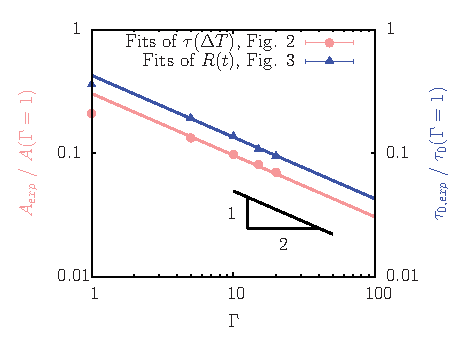
\includegraphics{epl17032f5_pr.eps}
\caption{(Colour on-line) Fitting parameters $A_{\textit{exp}}$ and $\tau_{0,\textit{exp}}$ normalized by the theoretical value of $A$ and $\tau_0$ when $\Gamma=1$ as a function of the reduced gravity $\Gamma$. We present the data coming from the fit of the lifetime as a function of the temperature (fig.~\ref{epl17032fig2}, red circles-left scale) and the data coming from the fit of the evolution of the radius with time for drops on a substrate at $300\un{^\circ C}$, where $A$ varies only through $\Gamma$ (fig.~\ref{epl17032fig3}, blue triangles-right scale).} \label{epl17032fig5}
\end{figure}

Fits of the lifetime data of fig.~\ref{epl17032fig2} with a power law, \textit{i.e.} $A_{\textit{exp}}\Delta T^{-3/4}$, allow to test this hypothesis. The theoretical value of $A(\Gamma=1)$ is $46256\un{s\cdot K^{3/4}}$. The values of $A_{\textit{exp}}$ normalized by $A(\Gamma=1)$ are reported as a function of the reduced gravity in fig.~\ref{epl17032fig5} (red circles-left scale). The plain red line indicates the slope $\Gamma^{-1/2}$, in very good agreement with experiments. The prefactor of the theory seems to be slightly overestimated, however. The good agreement between the theory and the experiments is also illustrated by the values of $\tau_{0,\textit{exp}}$ obtained by fitting the evolution of the radius with time for drops on a substrate at $300\un{^\circ C}$ by eq.~(\ref{epl17032eqn2}) (blue triangles-right scale). These values are normalized by the theoretical value of $\tau_0$ at $1g$ which is equal to 870\un{s}. According to eq.~(\ref{epl17032eqn4}), all the data should collapse on the same $\Gamma^{-1/2}$ curve, in good agreement with observations.

\subsection{Chimneys}

Large puddles were also investigated \nobreak{under} high-gravity conditions. The annulus located on the hot plate was completely filled with water. Many chimneys appear in these Leidenfrost puddles. By imaging, we measured $D_{ch}$, the distance between two adjacent chimneys from center to center, as a function of the gravity. This was done by measuring this distance for around a hundred pairs of chimneys. The cumulative distribution function of these measurements is typical of a Gaussian distribution of the distances. This enabled us defining a mean distance and a standard deviation. The results are reported in fig.~\ref{epl17032fig6}. The continuous line is a fit with a power law $D_{ch}=7.89\ a \propto \Gamma ^{-1/2}$.

\begin{figure}%f6
\centering
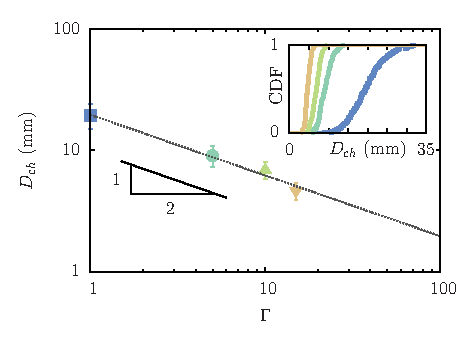
\includegraphics{epl17032f6_pr.eps}
\caption{(Colour on-line) Distance between adjacent chimneys $D_{ch}$ as a function of the reduced gravity $\Gamma$. The temperature of the substrate is $300\un{^\circ C}$. The dashed line is a power law fit with exponent $-1/2$. The inset represents the CDF of $D_{ch}$ for each reduced gravity.} \label{epl17032fig6}
%\vspace*{-4.2pt}
\end{figure}

This behaviour can be explained on the basis of the arguments developed in ref.~\cite{epl17032bib3}. The chimneys are due to a Rayleigh-Taylor--like instability of the vapor film. The instability characteristic length can be determined by triggering the instability with a small sinusoidal perturbation. In doing so, the critical radius above which chimneys are observed, $R_{c}$, is found to be linked with the height of the puddle $h=2\ a$, namely $R_c=3.84\ a$~\cite{epl17032bib3}. In their study of a drop levitating over blown air, Snoeijer \textit{et~al.} find a maximum stable radius $R_c \simeq 3.95\ a$.\cite{epl17032bib4}, a close value indeed. The distance between adjacent chimneys is not the same quantity as $R_c$, but appears to be slightly above twice the critical radius found in experiments and theory~\cite{epl17032bib3,epl17032bib4,epl17032bib8}.

\subsection{Leidenfrost point}

Despite the fact that the Leidenfrost effect has been studied extensively for some time, the description of the physical mechanisms that determine the Leidenfrost point is not complete. It is commonly defined as the temperature of the substrate at which the total evaporation time of a drop on a substrate above the~boiling point is the longest~\cite{epl17032bib3,epl17032bib19,epl17032bib20,epl17032bib23,epl17032bib27}. However, its dependence on parameters such as the thermal \nobreak{properties} of the substrate, the nature of the liquid or the relative humidity is still unclear. In particular, the disruption of the film occur at higher temperature on rough substrates~\cite{epl17032bib20,epl17032bib21,epl17032bib22,epl17032bib23}, but superhydrophobic substrates that are rough \textit{per~se} are characterized by a lower Leidenfrost point~\cite{epl17032bib24}, just as for rough hydrophobic substrates~\cite{epl17032bib25}.

From there we decided to take advantage of the LDC to study the influence of the gravity on the Leidenfrost point. A small but systematic shift of the Leidenfrost point is observed when the gravity is increased, \textit{i.e.} from $225\un{^\circ C}$ at $\Gamma=1$ to $240\un{^\circ C}$ at $\Gamma=20$, as illustrated in fig.~\ref{epl17032fig7}.

\begin{figure}%f7
\centering
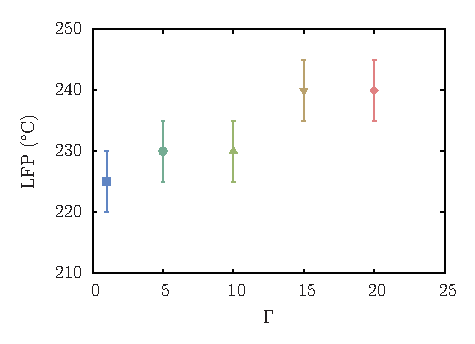
\includegraphics{epl17032f7_pr.eps}
\caption{(Colour on-line) The Leidenfrost point with respect to the reduced gravity $\Gamma$.} \label{epl17032fig7}
%\vspace*{-4.2pt}
\end{figure}

The large uncertainties originate from the temperature step between two points in fig.~\ref{epl17032fig2}. However, smaller steps would not have decreased the uncertainties drastically because, at these scales, the cooling of the substrate between the Leidenfrost drops may become significant and difficult to estimate.

Even though it is not possible to extract some scaling, a qualitative reasoning is possible. It can intuitively be expected that the Leidenfrost effect takes place when the vapor film is thick enough to prevent any contact between the liquid drop and the substrate. Under the hypothesis of a flat drop bottom, the thickness of the vapor film under a puddle~\cite{epl17032bib3} reads
\begin{equation}%eq5
h=\left(\frac{3\kappa_v\Delta T\eta_v}{4L\rho_v\rho\Gamma ga}\right)^{1/4}R^{1/2}.
\label{epl17032eqn5}
\end{equation}

Focusing on the role of gravity and temperature one can then find, for a given volume of liquid $V \simeq2\pi R^2a$, that the thickness of the vapor film depends indeed on the plate temperature $h\sim\Delta T^{1/4} $, but not anymore on the reduced gravity. Then, if it is assumed that this thickness needs to be higher than some threshold value for the film not to be disrupted, no effect of gravity on the Leidenfrost point is expected.

Figure~\ref{epl17032fig7} indicates however that the critical temperature does slightly increase with the gravity level, pointing to a need for a more accurate description of the vapor layer.

Considering the model of Sobac~\textit{et~al.}~\cite{epl17032bib8}, we see indeed that the film is not flat and that the {minimum} thickness of the vapor film, at the so-called neck, does decrease significantly (25{\%}) with the reduced gravity (inset of fig.~\ref{epl17032fig4}). This would imply a larger temperature to maintain $h_{\textit{neck}}$ above a threshold value and avoid contact between the drop and the plate, and thus a larger Leidenfrost point. This refined model is thus qualitatively consistent with the observations in fig.~\ref{epl17032fig7}. Note however that this aspect needs to be studied further. In particular, it appears that the rate of decrease of $h_{\textit{neck}}$ with $\Gamma$ is strongly dependent upon the volume of the droplet, which, moreover, continuously decreases during the evaporation process. It is therefore impossible to characterize it by a single scaling law, and the prediction of the Leidenfrost point might therefore require more advanced models to be developed.

\section{Conclusion}

Leidenfrost drops were studied in a variable-gravity environment between~1 and~20\un{times} the Earth gravity. The evaporation dynamics was studied by imaging the apparent radius of the drop with time, and by measuring the lifetime of a drop \textit{vs.} temperature. Simple modeling in terms of classical scalings\cite{epl17032bib3} satisfactorily rationalizes experiments, \textit{e.g.} in terms of drop lifetime and shape modification. More surprisingly, we found that the Leidenfrost point is slightly shifted towards larger temperatures as the gravity is increased. Even though this effect is not fully understood, it appears that explaining it might require the detailed thickness profile of the vapor film to be taken into account.

\acknowledgments{SD, PC, and MB thank F.R.S.-FNRS for financial support (the first two for their Senior Research Associate position, and MB for his FRIA fellowship).~This research has been funded by the Interuniversity Attraction Pole Programme (IAP 7/38 MicroMAST) initiated by the Belgian Science Policy Office, and by the ODILE FRFC 2.4623 project initiated by F.R.S.-FNRS.~The authors thank ESA and ELGRA for allowing the access to the LDC facility throughout the project. The authors thank the ``Spin Your Thesis'' program.~A-LB thanks the ANR through \textit{Freeflow} project for financial support. The authors would also like to warmly thank M. \textsc{M\'elard} and \textsc{S. Rondia} for the experimental setup.}

\begin{thebibliography}{99}

\bibitem{epl17032bib1}
\Name{Gottfried B., Lee C. \and Bell K.}
\REVIEW{Int. J. Heat Mass Transfer}{9}{1966}{1167}.

\bibitem{epl17032bib2}
\Name{Leidenfrost J.~G.}
\Book{De Aquae Communis Nonnullis Qualitatibus Tractatus}
\Publ{Duisburg}
\Year{1756}.

\bibitem{epl17032bib3}
\Name{Biance A.-L., Clanet C. \and Qu\'er\'e D.}
\REVIEW{Phys. Fluids}{15}{2003}{1632}.\vadjust{\vspace*{5.45pc}\pagebreak}

\bibitem{epl17032bib4}
\Name{Snoeijer J.~H., Brunet P. \and Eggers J.}
\REVIEW{Phys. Rev.~E}{79}{2009}{036307}.

\bibitem{epl17032bib5}
\Name{Myers T.~G. \and Charpin J. P.~F.}
\REVIEW{Phys. Fluids}{21}{2009}{063101}.

\bibitem{epl17032bib6}
\Name{Pomeau Y., Le~Berre M., Celestini F. \and Frisch~T.}
\REVIEW{C. R. Mec.}{340}{2012}{867}.

\bibitem{epl17032bib7}
\Name{Xu X. \and Qian T.}
\REVIEW{Phys. Rev. E}{87}{2013}{043013}.

\bibitem{epl17032bib8}
\Name{Sobac B., Rednikov A., Dorbolo S. \and Colinet P.}
\REVIEW{Phys. Rev. E}{90}{2014}{053011}.

\bibitem{epl17032bib9}
\Name{Burton J.~C., Sharpe A.~L., van~der Veen R. C.~A., Franco A. \and Nagel S.~R.}
\REVIEW{Phys. Rev. Lett.}{109}{2012}{074301}.

\bibitem{epl17032bib10}
\Name{Duchemin L., Lister J.~R. \and Lange U.}
\REVIEW{J. Fluid Mech.}{533}{2005}{161}.

\bibitem{epl17032bib11}
\Name{Lister J.~R., Thompson A.~B., Perriot A. \and Duchemin L.}
\REVIEW{J. Fluid Mech.}{617}{2008}{167}.

\bibitem{epl17032bib12}
\Name{Eggers J., Fontelos M.~A., Josserand C. \and \nobreak{Zaleski} S.}
\REVIEW{Phys. Fluids}{22}{2010}{062101}.

\bibitem{epl17032bib13}
\Name{Biance A.-L., Pirat C. \and Ybert C.}
\REVIEW{Phys. Fluids}{23}{2011}{022104}.

\bibitem{epl17032bib14}
\Name{Tran T., Staat H. J.~J., Prosperetti A., Sun C. \and Lohse D.}
\REVIEW{Phys. Rev. Lett.}{108}{2012}{036101}.

\bibitem{epl17032bib15}
\Name{Lastakowski H., Boyer F., Biance A.-L., Pirat C. \and Ybert C.}
\REVIEW{J. Fluid Mech.}{747}{2014}{103}.

\bibitem{epl17032bib16}
\Name{Linke H., Alem\'an B.~J., Melling L.~D., Taormina M.~J., Francis M.~J., Dow-Hygelund C.~C., Narayanan V., Taylor R.~P. \and Stout A.}
\REVIEW{Phys. Rev. Lett.}{96}{2006}{154502}.

\bibitem{epl17032bib17}
\Name{Dupeux G., Le Merrer M., Lagubeau G., Clanet C., Hardt S. \and Qu\'er\'e D.}
\REVIEW{EPL}{96}{2011}{58001}.

\bibitem{epl17032bib18}
\Name{Hashmi A., Xu Y., Coder B., Osborne P.~A., \nobreak{Spafford} J., Michael G.~E., Yu G. \and Xu~J.}
\REVIEW{Sci. Rep.}{2}{2012}{797}.

\bibitem{epl17032bib19}
\Name{Bernardin J.~D. \and Mudawar I.}
\REVIEW{Trans. ASME}{121}{1999}{894}.

\bibitem{epl17032bib20}
\Name{Kim H., Truong B., Buongiorno J. \and Hu L.-W.}
\REVIEW{Appl. Phys. Lett.}{98}{2011}{083121}.

\bibitem{epl17032bib21}
\Name{Kim S.~H., Ahn H.~S., Kim J., Kaviany M. \and Kim M.~H.}
\REVIEW{Appl. Phys. Lett.}{102}{2013}{233901}.

\bibitem{epl17032bib22}
\Name{Tran T., Staat H. J.~J., Susarrey-Arce A., \nobreak{Foertsch} T.~C., van Houselt A., Gardeniers H.~J.~G.~E., Prosperetti A., Lohse D. \and Sun C.}
\REVIEW{Soft Matter}{9}{2013}{3272}.

\bibitem{epl17032bib23}
\Name{Kruse C., Anderson T., Wilson C., Zuhlke C., Alexander D., Gogos G. \and Ndao S.}
\REVIEW{Langmuir}{29}{2013}{9798}.

\bibitem{epl17032bib24}
\Name{Vakarelski I.~U., Patankar N.~A., Marston J.~O., Chan D. Y.~C. \and Thoroddsen S.~T.}
\REVIEW{Nature}{489}{2012}{274}.

\bibitem{epl17032bib25}
\Name{Arnaldo~del Cerro D., Mar\'in A.~G., R\"omer G.~R.~B.~E., Pathiraj B., Lohse D. \and in~'t Veld A.~H.}
\REVIEW{Langmuir}{28}{2012}{15106}.

\bibitem{epl17032bib26}
\Name{de~Gennes P.-G., Brochard-Wyart F. \and Qu{\'e}r{\'e} D.}
\Book{Gouttes, bulles, perles et ondes}
\Publ{Belin Paris}
\Year{2002}.

\bibitem{epl17032bib27}
\Name{Wang A.-B., Lin C.-H. \and Chen C.-C.}
\REVIEW{Phys. Fluids}{12}{2000}{1622}.

\end{thebibliography}

\end{document}




